\section{Training Framework}
\label{sec:agentic_training_framework}

The goal of this section is to utilize Reinforcement Learning (RL) to train the agent defined in Section~\ref{sec:tree_based_agentic_reasoning}(Section~\ref{sec:tree_based_agentic_reasoning}). 
To this end, we adopt a multi-turn Reinforcement Learning (RL) paradigm (Section~\ref{subsec:multi_turn_rl}).
However, directly optimizing this framework faces a fundamental challenge: \textit{reward sparsity}. This arises from two coupled factors: the strict syntactic requirements of agentic reasoning (where invalid actions yield no feedback) and the binary nature of table correctness (where near-misses yield zero reward).
To address these challenges, we propose two modules: a \textit{Cold-Start Curriculum} (Section~\ref{subsec:cold_start}) designed to initialize the basic ability to agentic tree-based reasoning, and a \textit{Hybrid Reward} mechanism (Section~\ref{subsec:reward}) to densify learning signals for RL optimization.

\subsection{Multi-turn Reinforcement Learning}
\label{subsec:multi_turn_rl}

\noindent \textbf{GRPO.} 
We adopt the Group Relative Policy Optimization (GRPO) algorithm~\cite{shao2024deepseekmath} to optimize the agent's policy $\pi_\theta$. Unlike traditional PPO~\cite{schulman2017proximal} which requires a separate value function critic (often computationally expensive for long-context reasoning), GRPO estimates the baseline directly from group statistics.
Formally, given an ADP task input $x = (\mathcal{D}, \mathcal{S}) \sim D$, we generate a group of $G$ trajectories (rollouts) $\tau = \{y_i\}_{i=1}^G$ sampled from the current policy $\pi_{\theta_{\text{old}}}$.
For each trajectory $y_i$, we compute an advantage $A_i$ based on the reward function. The policy is optimized by maximizing the following objective:
\begin{equation}
\begin{split}
\mathcal{J}(\theta) = \mathbb{E}_{x \sim D, \{y_i\}_{i=1}^G \sim \pi_{\theta_{\text{old}}}(\cdot|x)} 
\frac{1}{G} \sum_{i=1}^G \bigg[ \min \bigg( \frac{\pi_\theta(y_i|x)}{\pi_{\theta_{\text{old}}}(y_i|x)} A_i, \\
\text{clip} \left( \frac{\pi_\theta(y_i|x)}{\pi_{\theta_{\text{old}}}(y_i|x)}, 1-\epsilon, 1+\epsilon \right) A_i \bigg) - \beta \mathbb{D}_{\text{KL}} (\pi_\theta || \pi_{\theta_{\text{ref}}}) \bigg]
\end{split}
\end{equation}
where $\epsilon$ is the clipping parameter to constrain the policy update, and $\pi_{\theta_{\text{ref}}}$ is the reference policy (typically the SFT model) used to prevent reward hacking via a KL-divergence penalty.

\noindent \textbf{Masking Observations.} 
In our agentic framework, a trajectory $y_i$ is a sequence of interleaved tokens consisting of the agent's reasoning (actions) and the environment's feedback (observations).
The environment feedback, encapsulated within the \texttt{<observe} tags (i.e., the serialized tree state $p$), represents the deterministic output of the execution engine, not the generative capability of the model.
Therefore, we apply a binary mask to the loss function. We zero out the gradients for all tokens belonging to the observation segments, ensuring that the policy $\pi_\theta$ is trained strictly on its decision-making outputs (e.g., content within \texttt{<plan}, \texttt{<expand}, and \texttt{<terminate} tags).

\stitle{Challenges of Sparsity.} 
Directly applying RL to ADP is non-trivial due to two compounding sources of sparsity:

\noindent(C1) \textbf{Syntactic Invalidity.} In the early stage of training, the agent frequently generates structurally malformed outputs, such as undefined action tags, hallucinated operator names, or incorrect argument types. Such failures trigger immediate exceptions in the execution engine, resulting in aborted trajectories that provide no meaningful learning signal regarding the data preparation logic.

\noindent(C2) \textbf{Outcome Sparsity.} Even when the pipeline is executable, the task success is strictly binary: the generated table $\hat{T}$ must exactly match the ground truth $T^*$. This outcome-based supervision ignores ``near-miss'' trajectories (e.g., a pipeline that performs correct cleaning and joins but fails due to a single column renaming error), rendering credit assignment inefficient over long horizons.

\subsection{Cold-Start Curriculum}
\label{subsec:cold_start}

%!TEX root = ../../main.tex
\begin{figure*}[t]
    \centering 
    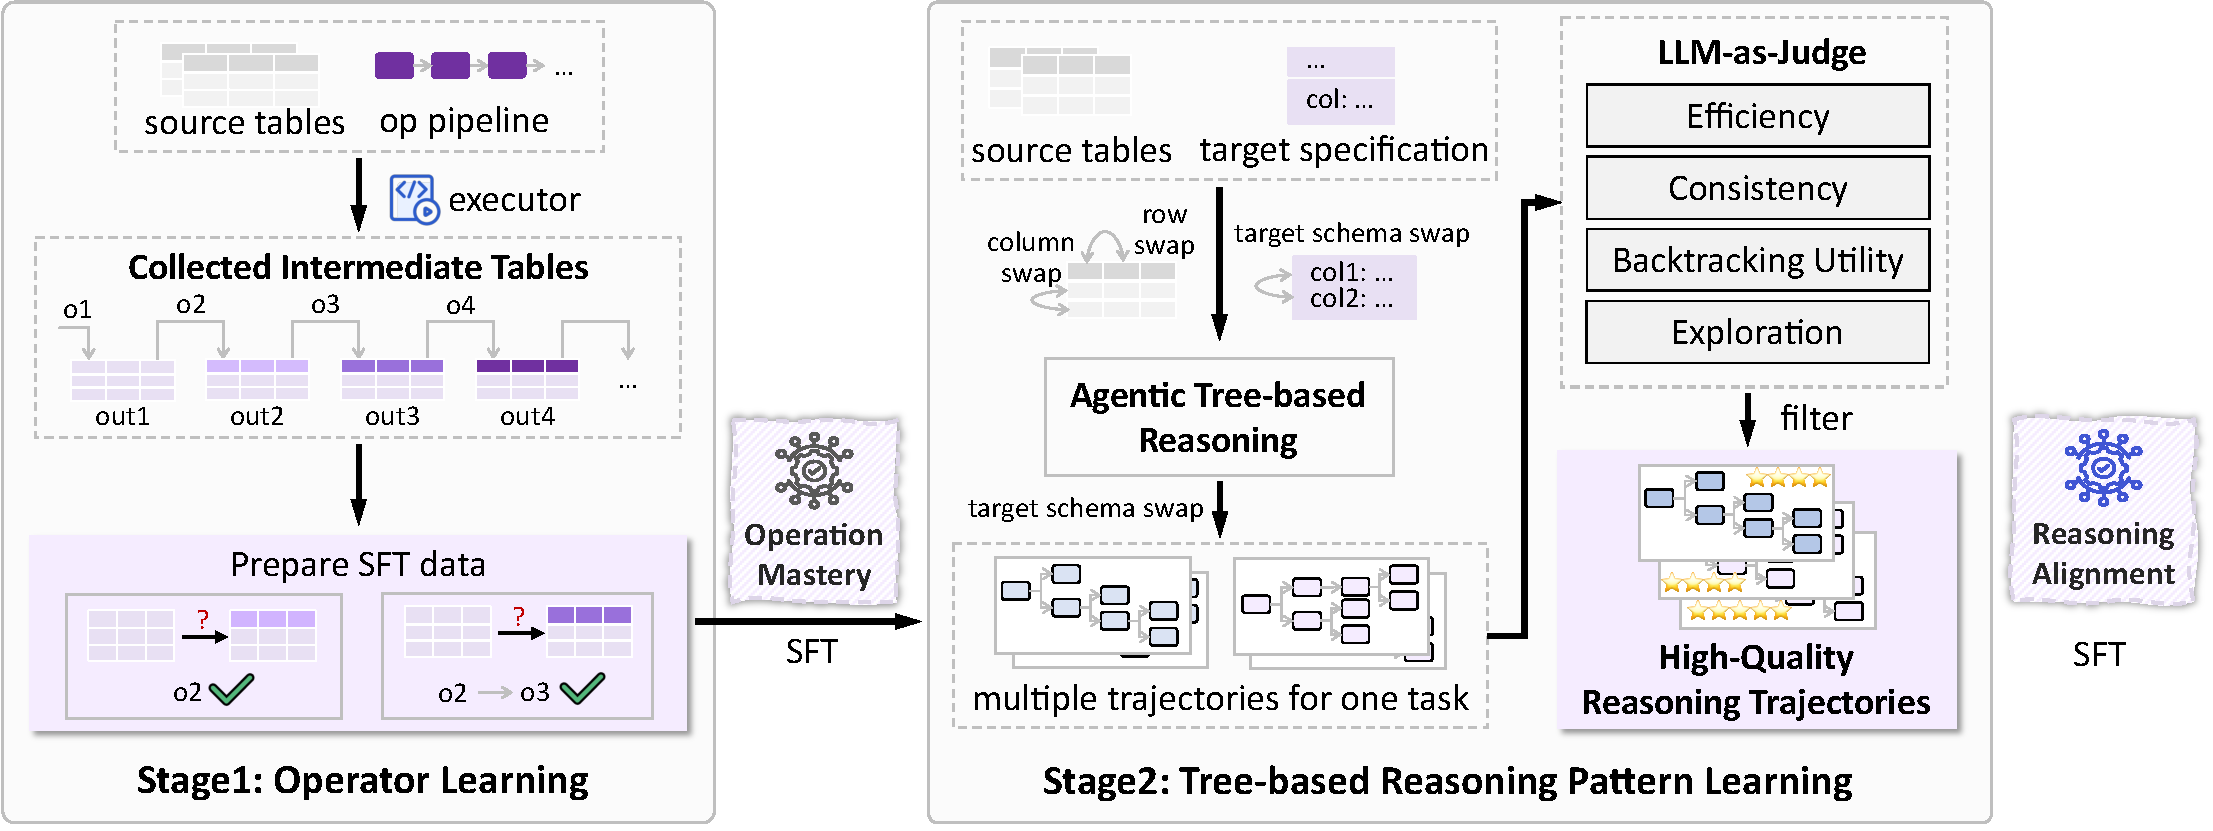
\includegraphics[width=0.9\textwidth]{figures/fig/cold_start.pdf}
  % \vspace{-0.7em}
    \caption{Overview of the progressive cold-start curriculum, which consists of two stages: Operator Learning and Multi-Solution Generation. An LLM-as-Judge mechanism filters these trajectories to ensure high-quality supervision for fine-tuning.
    }
    \label{fig:cold_start}
  % \vspace{-1em}
\end{figure*}

To mitigate (C1) Syntactic Invalidity, we design a two-stage curriculum, as illustrated in Figure~\ref{fig:cold_start}, that bootstraps the agent's understanding of both atomic operators and the reasoning protocol defined in Section~\ref{sec:tree_based_agentic_reasoning}.

\stitle{Operator Learning.}
We first focus on the syntax and semantics of individual operators.
As shown in Figure~\ref{fig:cold_start}, we employ a sub-sequence modeling strategy: given source tables and a ground-truth operator pipeline $\Pi_{\text{total}}$, we first execute the operators sequentially to collect intermediate tables. Then, we sample a contiguous sub-sequence $\Pi_{\text{sub}} = (o_i, \dots, o_{i+k})$ with corresponding source tables and generated table(s). 
The model is then trained via Supervised Fine-Tuning (SFT) to reconstruct $\Pi_{\text{sub}}$ conditioned on the input-output pair:
$$
\mathcal{L}_{\text{op}}(\theta) 
= - \sum_{(T_{\text{in}}, T_{\text{out}}, \Pi_{\text{sub}}) \in \mathcal{D}_{\text{op}}}
\log P_\theta(\Pi_{\text{sub}} \mid T_{\text{in}}, T_{\text{out}}).
$$
This stage allows the model to master operator function signatures and argument formats, isolating execution logic from complex planning.

\stitle{Tree-Based Reasoning Pattern Learning.}
This stage aligns the agent with the \textit{Agentic Tree-based Reasoning} protocol, specifically the usage of tags like \texttt{<plan} and \texttt{<expand}.

The right part of Figure~\ref{fig:cold_start} illustrates how we construct a dataset of high-quality reasoning trajectories by distilling from strong teacher models (e.g., DeepSeek-R1).
To ensure robustness, we apply input perturbations $\Phi$ (e.g., shuffling row/column orders or paraphrasing $\mathcal{S}$) to the training data and generate a set of candidate trajectories:
$$
\mathcal{U}_{cand} = \{\tau_k \mid \tau_k \sim \pi_{teacher}(\Phi(\mathcal{D}, \mathcal{S})), \;\; k=1,\dots,K\}.
$$
To filter out suboptimal reasoning, we employ an \textit{LLM-as-a-Judge} scoring function $Q(\tau)$ that evaluates the trajectory based on four dimensions: (1) \textit{Efficiency} (penalizing redundant steps), (2) \textit{Consistency} (alignment between \texttt{<plan} thoughts and \texttt{<expand} actions), (3) \textit{Backtracking Utility} (whether rollbacks successfully resolved errors), and (4) \textit{Exploration} (diversity of visited nodes).
$$
Q(\tau) = \sum w_d \cdot f_d(\tau),
$$
where $w_d$ are weighting coefficients and $f_d(\cdot)$ are normalized scoring sub-functions.
We retain the top-ranked trajectories $\mathcal{U}_{filtered} = \{\tau \in \mathcal{U}_{cand} \mid Q(\tau) \ge \delta\}$ and perform SFT to minimize the negative log-likelihood of the actions $a_t$ given the tree state $\mathcal{T}_t$:
$$
\mathcal{L}_{\text{tree}}(\theta)
= - \sum_{\tau \in \mathcal{U}_{filtered}}
\sum_{t=1}^{|\tau|} \log P_\theta(a_t \mid \mathcal{T}_t).
$$

\subsection{Hybrid Reward Design}
\label{subsec:reward}

\fmh{RL+Reward as subsection.}

To address (C2) Outcome Sparsity, we design a hybrid reward that densifies the feedback signal by acknowledging partial progress and reasoning quality.
We now define the reward $ R(\tau) $ used in Section~\ref{subsec:multi_turn_rl}.

\stitle{Outcome Reward ($R_{\text{out}}$).}
This is the strict success signal triggered when the agent executes \texttt{<terminate}. Let $\hat{T}(\tau)$ be the table produced by the final pipeline $\Pi$ extracted from trajectory $\tau$, and $T^*$ be the ground truth.
$$
R_{\text{out}}(\tau) = \mathbb{I}(\hat{T}(\tau) \equiv T^*),
$$
where $\mathbb{I}(\cdot)$ is the indicator function.

\stitle{Partial Reward ($R_{\text{partial}}$).}
To guide the agent towards the correct solution during exploration, we quantify the similarity between $\hat{T}$ and $T^*$ across three dimensions:
(1) {Schema Alignment} ($S_{sch}$): The Jaccard similarity of column names.
(2) {Shape Consistency} ($S_{shp}$): A binary indicator of whether row counts match.
(3) {Content Fidelity} ($S_{cnt}$): The average column-wise similarity.
$$
R_{\text{partial}}(\tau) = \frac{1}{3}(S_{sch} + S_{shp} + S_{cnt}).
$$

\stitle{LLM-As-Judge Reward ($R_{\text{llm}}$).}
To discourage \textit{reward hacking}~\cite{taylor2025school} (e.g., the agent merely renames columns to boost $S_{sch}$ without actual cleaning), we reuse the quality assessment function $Q(\tau)$ defined in Section~\ref{subsec:cold_start} as a dense reward signal. This explicitly evaluates the quality of the content within \texttt{<plan} tags, encouraging the agent to maintain logical coherence even when the final data output is imperfect.


Finally, the total reward $R(\tau)$ used to update the policy via GRPO is the weighted sum of these components:
$$
R(\tau) = \alpha \cdot R_{\text{out}}(\tau) + \beta \cdot R_{\text{partial}}(\tau) + \gamma \cdot R_{\text{llm}}(\tau),
$$
where $\alpha, \beta, \gamma$ are hyperparameters balancing strict correctness, partial progress, and reasoning quality.

